\chapterimage{img/SuperKK.jpg} % Chapter heading image
\chapterspaceabove{6.75cm} % Whitespace from the top of the page to the chapter title on chapter pages
\chapterspacebelow{7.25cm} % Amount of vertical whitespace from the top margin to the start of the text on chapter pages

%------------------------------------------------

\chapter{Neutrini}

\section{Produzione nel sole di neutrini}
Il principale meccanismo di produzione di neutrini all'interno di una stella, come il sole, è il meccanismo di fusione. Ad esempio i seguenti processi danno luogo alla produzione di neutrini
\begin{gather*}
    p + p \rightarrow d + e^+ + \nu_e \\
    4p \rightarrow ^4\textup{He} + 2e^+ + 2\nu_e.
\end{gather*}
In particolare si noti che la massa del nucleo prodotto ha una massa più piccola della massa totale dei reagenti, la massa in eccesso rende possibile la produzione di neutrini. A proposito di questo, si potrebbe studiare l'andamento del difetto di massa per nucleone costruendo la seguente funzione
\begin{equation*}
    f = \frac{(m_n(A-Z) + m_p Z - m_N)c^2}{A},
\end{equation*}
questa funzione è calcolabile per ogni nucleo $(A, Z)$, in particolare si veda Fig.(\ref{fig:nuclei}).
\begin{figure}[H]
    \centering
    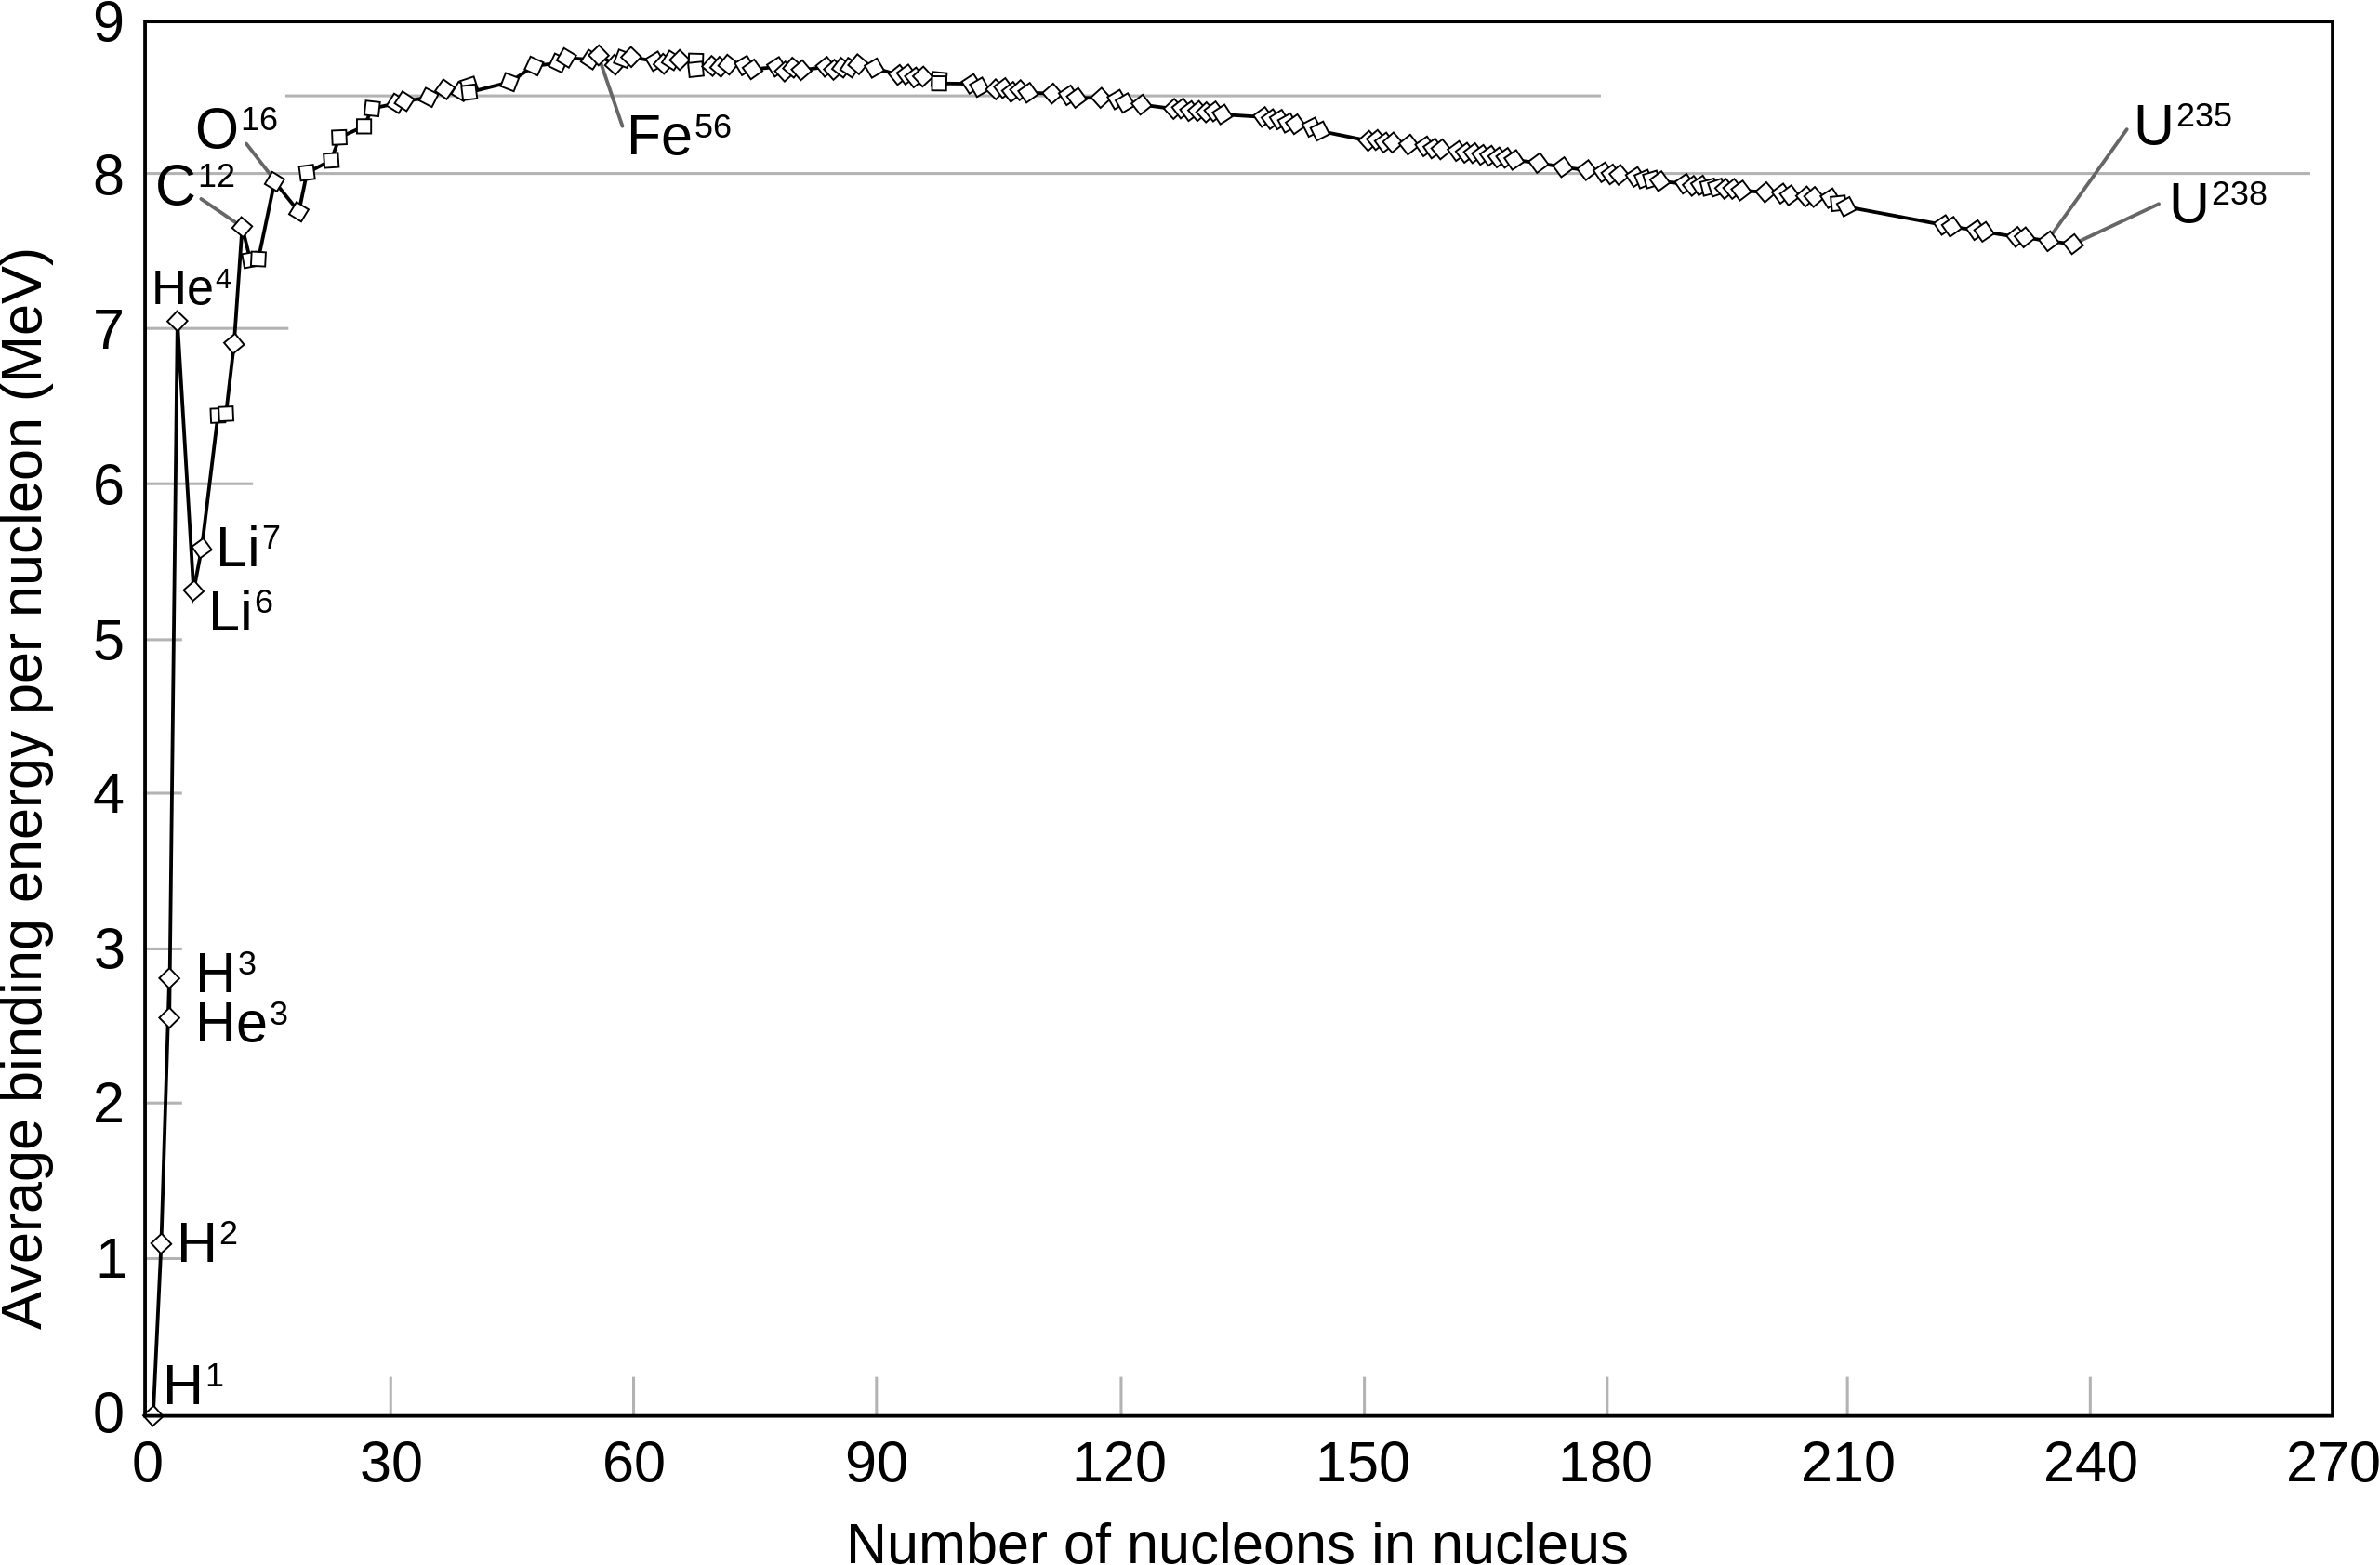
\includegraphics[width=0.5\textwidth]{img/nuclei.png}
    \caption{Andamento dell'energia media di legame per nucleone.}
    \label{fig:nuclei}
\end{figure}
Per far sì che avvenga il processo di fusione, i due protoni (o in generale i reagenti) devono vincere la repulsione coloumbiana, visualizzabile come una barriera di potenziale con legge $z_1 z_2 e^2 / r$, e raggiungere la distanza $r_0$ oltre la quale si ha una buca di potenziale ($0 < r < r_0$). Il valore del potenziale coulombiano a distanza $r_0$ lo chiameremo $B$ e per $r_0$ utilizzeremo una nota approssimazione del raggio nucleare, al di sotto della quale i reagenti possono interagire tramite interazione forte
\begin{gather*}
    B = \frac{z_1 z_2 e^2}{r_0},\\
    r_0 = A^{\frac{1}{3}}1\,\textup{fm}.
\end{gather*}
Se conosciamo l'energia cinetica dei protoni all'interno del sole possiamo determinare se i due protoni che si scontrano riescono a passare la barriera di potenziale o meno. Per fare dei conti numerici nel nostro caso basterebbe sostituire $z_1 = z_2 = A = 1$, otteniamo che $B = 1.5\,\textup{MeV}$. Vorremmo dunque ottenere l'energia cinetica dei protoni all'interno del sole. Per la precisione siamo interessati alla distribuzione in energia dei protoni all'interno del sole, che possiamo considerare distribuiti come una Maxwell-Boltzman
\begin{equation}
    f(E) \varpropto \sqrt{E} e^{-\frac{E}{kT}}\frac{1}{(kT)^{3/2}},\label{eq:maxwellbolz}
\end{equation}
ci interessa quindi ottenere una stima della temperatura all'interno del sole. L'idea da seguire è quella di imporre l'equilibrio idrostatico al sole, tra pressione del gas contenuto del sole e forza di attrazione gravitazionale del gas. Consideriamo un'area $\der S$ su di un guscio sferico del sole con raggio $r$ e spessore $\der r$
\begin{equation*}
    \begin{split}
        \frac{G m(r)\rho(r)\der S \der r}{r^2} & = \bigl(P(r) - P(r+\der r)\bigr)\der S\\
                                               & = -\frac{\der P}{\der r} \der r \der S,
    \end{split}
\end{equation*}
moltiplicando e dividendo il primo membro per $4\pi r^2$, possiamo aggiustare l'equazione come segue
\begin{equation}
    \frac{\der P}{\der m} = - \frac{Gm}{4\pi r^4}.
    \label{eq:sole1}
\end{equation}
Facciamo adesso una approssimazione al primo membro e assumiamo che la derivata sia costante, possiamo dunque sostituire il primo membro con il termine $\frac{P_\textup{c}}{M_\odot}$.
\begin{definition}
    Ciascuna grandezza relativa al sole viene sempre indicata con il pedice $\odot$. Ad esempio, riportiamo a scopo informativo i seguenti valori
    \begin{gather*}
        M_\odot = 2 \times 10^{30}\,\textup{kg},\\
        R_\odot = 0.7 \times 10^{9} \,\textup{m}.
    \end{gather*}
\end{definition}
Per approssimare il secondo membro di Eq.(\ref{eq:sole1}) possiamo supporre che in un volume corrispondente a metà del raggio sia contenuta metà della massa del sole. Dunque riscriviamo Eq.(\ref{eq:sole1}) come
\begin{equation}
    P_\textup{c} = \frac{G M_\odot^2}{R_\odot^4}\frac{2}{\pi}.
    \label{eq:pressione_sole}
\end{equation}
Dobbiamo dunque scrivere una equazione di stato per il gas contenuto nel sole, volendo correlare la pressione alla temperatura
\begin{equation*}
    PV = nkT = \sum_i n_i(Z_i + 1)kT,
\end{equation*}
dove al secondo passaggio abbiamo esplicitato le diverse specie che compongono il gas, ovvero protoni e elettroni. Con semplici considerazioni, possiamo riscrivere $n_i$ come seguente
\begin{equation*}
    n_i = \frac{\rho_i V N_\textup{A}}{A_i} = \frac{\rho_i}{\rho}\frac{N_\textup{A}}{A_i} \equiv x_i \frac{N_\textup{A}}{A_i}.
\end{equation*}
Sostituiamo dunque $n_i$ come ricavato adesso nella equazione di stato del gas e otteniamo 
\begin{equation}
    PV = \sum_i \frac{x_i (1 + Z_i)}{A_i}N_\textup{A} k T = \overline{n}\mathcal{R}T,
    \label{eq:pressione_sole2}
\end{equation}
dove $\mathcal{R} = N_\textup{A}k$ è la costante dei gas perfetti, $\overline{n}$ è il numero medio di moli per nucleone. Nel caso di una singola specie (di protoni) otteniamo $\overline{n} = 2$. Mettiamo dunque insieme Eq.(\ref{eq:pressione_sole}) e Eq.(\ref{eq:pressione_sole2}) nella quale sostituiamo $V$ con $1 / \rho_c$. Inoltre anticipiamo che maggioreremo il fattore $1 / \rho_c$ con il reciproco della pressione media $(\frac{4}{3} \pi R_\odot ^3) / M_\odot$. Otteniamo la seguente espressione per la temperatura al centro del sole
\begin{equation*}
    T_\textup{c} \leq \frac{4}{3}\frac{GM_\odot}{\mathcal{R}R_\odot} \simeq 3 \times 10^{7} \, ^\circ \textup{K}.
\end{equation*}
Possiamo dunque ricavare l'energia cinetica media delle particelle all'interno del sole1
\begin{equation*}
    E_\textup{kin} = \frac{3\times 10^7\,\textup{°K}}{1.2\times 10^4 \,\textup{eV}} \simeq 2.5\,\textup{keV}.
\end{equation*}
Considerando che la distribuzione di probabilità vista prima dipendeva da $e^{-E/kT}$ otteniamo che questo fattore vale circa $e^{-1.5\,\textup{MeV} / 2.5\,\textup{keV}}$, ovvero un fattore $\sim e^{-1000} \sim 10^{-400}$, questa ricordiamo essere la probabilità di attraversare la barriera coulombiana. Possiamo ottenere una stima di quanti nucleoni fondono semplicemente moltiplicando il numero ottenuto per il numero totale di nucleoni $N_\textup{N} \simeq M_\odot N_\textup{A} \simeq 1.2 \times 10^{57}$, il numero di nucleoni che fondono rimane comunque circa $0$. L'unica maniera che abbiamo di vedere un processo di fusione dunque è quello di considerare l'attraversamento della barriera per effetto tunnel
\begin{equation*}
    \Pr(\textup{effetto tunnel}) = \exp \biggl( \displaystyle\int_{r_0}^{r_1} \sqrt{\frac{2m}{\hslash ^2}\bigl( V(r) - \overline{E} \bigr)} \der r \biggr),
\end{equation*}
risolviamo dunque l'integrale come seguente
\begin{equation*}
    \begin{split}
        \displaystyle\int_{r_0}^{r_1} \sqrt{\frac{2m}{\hslash ^2}\bigl( V(r) - \overline{E} \bigr)} \der r & = \sqrt{\frac{2m}{\hslash ^2}z_1 z_2 e^2} \int_{r_0}^{r_1} sqrt{\frac{1}{r_0} - \frac{1}{r_1}} \der r \\
        & = (\dots) \frac{1}{\sqrt{r_1}} \int_{r_0}^{r_1} \sqrt{\frac{r_1}{r_0} - 1} \frac{\der r}{r_1} r_1 \\
        & = (\dots) \sqrt{r_1} \int_{r_0 / r_1}^{1} \sqrt{\frac{1}{x} - 1} \der x = (\dots) \sqrt{r_1} \frac{\pi}{2},
    \end{split}
\end{equation*}
dove per risolvere l'ultimo integrale abbiamo approssimato l'estremo inferiore come seguente
\begin{equation*}
    \begin{cases}
        B = \frac{z_1 z_2 e^2}{r_0} \\
        \overline{E} = \frac{z_1 z_2 e^2}{r_1} 
    \end{cases}
    \Rightarrow \frac{r_0}{r_1} = \frac{\overline{E}}{B} \simeq 0.
\end{equation*}
Possiamo dunque scrivere la probabilità di attraversamento della barriera per effetto tunnel come seguente
\begin{equation}
    \Pr (\textup{effetto tunnel}) = \exp \biggl( -\pi \sqrt{\frac{2m}{\hslash^2} \frac{(z_1 z_2 e^2)^2}{\overline{E}}}\biggr) \equiv e^{-\sqrt{\frac{E_\textup{G}}{\overline{E}}}}.\label{eq:gamow} 
\end{equation}
\begin{definition}[Energia di Gamow]
    Il termine $E_\textup{G}$ che compare in Eq.(\ref{eq:gamow}) viene chiamata \emph{energia di Gamow}
    \begin{equation*}
        E_\textup{G} = \frac{2m_\textup{r}\pi^2}{\hslash^2}(z_1 z_2 e^2)^2,
    \end{equation*}
    dove $m_\textup{r}$ è la massa ridotta delle due particelle con rispettivamente $z_1$ e $z_2$ unità di carica.
\end{definition}
Nel caso di protone-protone $E_\textup{G}$ vale circa $600\,\textup{keV}$. Considerando il valore prima ottenuto per l'energia media all'interno del sole $\sim 1 \,\textup{keV}$, otteniamo che la nuova probabilità di attraversamento della barriera vale circa $10^{-10}$, molto maggiore con il $10^{-400}$ di prima e sicuramente dà un numero di protoni che fondono sicuramente diverso da zero, dovendo moltiplicare per $10^{57}$ nucleoni.

Vogliamo adesso capire come misurare i neutrini provenienti dal sole e quanti aspettarsene. Scriviamo la sezione d'urto
\begin{equation*}
    \frac{\der N}{\der t \der V} = \frac{n(r)^2}{2} \sigma v_\textup{R},
\end{equation*}
dove $n(r)^2/2$ è un fattore che tiene di conto che proiettili e bersagli sono entrambi protoni, e il fattore 2 tiene di conto dell'identicità di queste due specie, $v_\textup{R}$ è la velocità relativa tra proiettile e bersaglio, $\sigma$ è la sezione d'urto per il processo di fusione. Notare che $n = n(r)$ poichè la densità di particelle sarà in generale una funzione del raggio, ci aspettiamo in particolare che la maggior parte delle particelle si trovi al centro del sole. Dunque vogliamo ricavare il rate di fusione, e successivamente di produzione di neutrini, al centro del sole. Se consideriamo $b$ il parametro d'impatto per il processo di fusione, dobbiamo richiedere che $b$ sia comparabile con il raggio nucleare medio affinchè il processo avvenga. Da questa considerazione proviamo a ricavare la sezione d'urto. Consideriamo il momento angolare
\begin{equation*}
    pb = l\hslash \Rightarrow b = l \frac{\hslash}{p},
\end{equation*}
per ottenere una stima della sezione d'urto \emph{geometrica} devo sommare su tutti i possibili momenti angolari
\begin{equation*}
    \sigma_\textup{G} = \pi \sum_l\bigl[ b^2(l+1) - b^2(l) \bigr] = \pi \biggl(\frac{\hslash}{p}\biggr)^2 \sum_l \bigl[ (l+1)^2 - l^2 \bigr] = \pi \biggl(\frac{\hslash}{p}\biggr)\sum_l[2l + 1].
\end{equation*}
La sommatoria dovrebbe andare da $0$ a $\infty$, ma siccome deve valere $b \leq r_0$, dobbiamo rispettrare la condizione $l \leq r_0 p /\hslash$. Possiamo in effetti dare una stima del termine a destra della disuguaglianza e otteniamo che $l \leq 10^{-2}$, conta cioè unicamente l'onda S. Aggiustando la sezione d'urto geometrica per proiettili di natura ondulatoria, si ottiene che 
\begin{equation*}
    \sigma_\textup{G} = \frac{4\pi \hslash^2}{2m \overline{E}} \sin2 \delta_0 (E) = \frac{S(\overline{E})}{\overline{E}}.
\end{equation*}
Il numeratore dell'ultima espressione viene anche chiamato \emph{fattore astrofisico}. Dunque adesso possiamo scrivere che
\begin{equation*}
    \frac{\der N}{\der t \der V} \varpropto n^2(r) \frac{S(E)}{E} e^{-\sqrt{E_\textup{G} / E}}\sqrt{E},
\end{equation*}
se adesso moltiplichiamo per la distribuzione di Maxwell-Boltzman Eq.(\ref{eq:maxwellbolz}), possiamo fare una media sull'energia
\begin{equation*}
    \begin{split}
        \frac{\der N}{\der t \der V} & \varpropto \int_0^\infty n^2(r) \frac{S(E)}{E} e^{-\sqrt{E_\textup{G} / E}}\sqrt{E}\sqrt{E} e^{-\frac{E}{kT}}\frac{1}{(kT)^{3/2}} \der E \\
        & \varpropto \frac{n^2}{(kT)^3}\int_0^\infty S(E) e^{-\biggl(\sqrt{\frac{E_\textup{G}}{E}} + \frac{E}{kT}\biggr)} \der E
    \end{split}
\end{equation*}
Il fattore astrofisico dipende in particolare dal tipo di nuclei coinvolti, che possono dar vita ad eventi di risonanza. Se assumiamo però che $S(E)$ vari poco possiamo semplificare i calcoli e risolvere l'integrale. L'argomento dell'esponenziale tra parentesi è composto da un termine lineare e uno iperbolico in $E$, dunque esiste una regione di valori intermedi di energia tra questi due regimi in cui l'argomento tra parentesi varrà meno. In questa stessa regione la funzione integranda vale il suo massimo valore (per via del segno negativo nell'esponenziale). Questo picco che raggiunge la funzione integranda si chiama \emph{picco di Gamow} (indichiamola con $E_0$), se questo è abbastanza stretto e se $S(E)$ non ha effetti di risonanza posso approssimare $S = S(E_0)$. Successivamente dobbiamo approssimare (al secondo ordine) la funzone seguente
\begin{equation*}
    -f(E) \equiv \sqrt{\frac{E_\textup{G}}{E}} + \frac{E}{kT},
\end{equation*}
studiando la derivata prima possiamo identificare $E_0$ come il suo punto di minimo. La posizione del picco di Gamow risulta essere
\begin{equation*}
    E_0 = \sqrt[3]{E_\textup{G}}\biggl( \frac{kT}{2} \biggr)^{2/3}
\end{equation*}
dunque
\begin{equation*}
    -f(E) = \frac{3E_0}{kT} \equiv \tau \Rightarrow \tau = 3 \sqrt[3]{\frac{E_\textup{G}}{4kT}} \simeq 12,
\end{equation*}
dove abbiamo introdotto la notazione della variabile $\tau$ e abbiamo calcolato il valore approssimato per il caso di protone-protone. Portiamo avanti i calcoli e otteniamo
\begin{equation*}
    -f(E_0)'' = \frac{3}{4}\sqrt{E_\textup{G}} E_0^{-\frac{5}{2}} = \frac{\tau}{2E_0^2},
\end{equation*}
la funzione $f$ in un intorno del punto $E_0$ è approssimabile come seguente
\begin{equation*}
    f(E) \simeq -\tau -\frac{\tau}{4E_0^2}(E - E_0)^2,
\end{equation*}
quindi l'integrale iniziale da valutare che mi dà il rate è 
\begin{equation*}
    R \varpropto \frac{n^2}{(kT)^{3/2}} \int_0^\infty e^{-\tau} e^{-\frac{\tau}{4E_0^2}(E-E_0)^2}\der E,
\end{equation*}
eseguiamo il seguente cambio di variabile
\begin{gather*}
    \frac{\sqrt{\tau}}{2E_0}(E-E_0) = \xi \\
    \der \xi = \frac{\sqrt{\tau}}{2E_0}\der E,
\end{gather*}
riprendendo l'integrale abbiamo
\begin{equation*}
    R \varpropto \frac{n^2}{(kT)^{3/2}} e^{-\tau} \frac{2E_0}{\sqrt{\tau}}\int_{-\sqrt{\tau}/2}^{\infty} e^{-\xi^2} \der \xi.
\end{equation*}
Approssimando l'integrale tra $-\infty$ a $+\infty$, possiamo riscrivere l'espressione del rate $R$
\begin{equation*}
    R \varpropto \frac{n^2}{(kT)^{3/2}}e^{-\tau}\frac{E_0}{\sqrt{\tau}},
\end{equation*}
esplicitiamo la dipendenza da $\tau$, osserviamo che la potenza rimanente è $\tau^2$
\begin{equation*}
    R \varpropto \tau^2 e^{-\tau},
\end{equation*}
questa in effetti ci dice la dipendenza dalla temperatura all'interno del sole per il rate di fusione, quindi per il rate di produzione di neutrini. Se vogliamo esprimere questa dipendenza come $T^{\nu}$, ne facciamo il logaritmo
\begin{equation*}
    \log R = \textup{cost} + \nu \log T \Rightarrow \nu = \frac{\partial \log R}{\partial \log T},
\end{equation*}
per quanto abbiamo scritto prima vale anche
\begin{equation*}
    \log R = \textup{cost} + 2 \log \tau - \tau
\end{equation*}
quindi
\begin{equation*}
    \frac{\partial \log R}{\partial \log T} = 2 \frac{\partial \log \tau}{\partial \log T} - \frac{\partial \tau}{\partial \log T} = (2 - \tau) \frac{\partial \log \tau}{\partial \log T},
\end{equation*}
dato che $\tau \varpropto T^{-1/3}$ e quindi $\log \tau = \textup{cost} - \frac{1}{3} \log T$, mettendo tutto insieme otteniamo che
\begin{equation*}
    \nu = \frac{\tau}{3} - \frac{2}{3},
\end{equation*}
nel caso di protone-protone sappiamo che $\tau = 12$, quindi $\nu \sim 3.3$. Volendo stimare la precisione con cui misuriamo il rate possiamo scrivere
\begin{equation*}
    \frac{\Delta R}{R} = \nu \frac{\Delta T}{T},
\end{equation*}
la dipendenza lineare da $\nu$ fa sì che, data la crescenza di $\nu$ per nuclei più pesanti, l'incertezza sul rate di neutrini sia maggiore.
